\begin{figure}[!h]
\centering
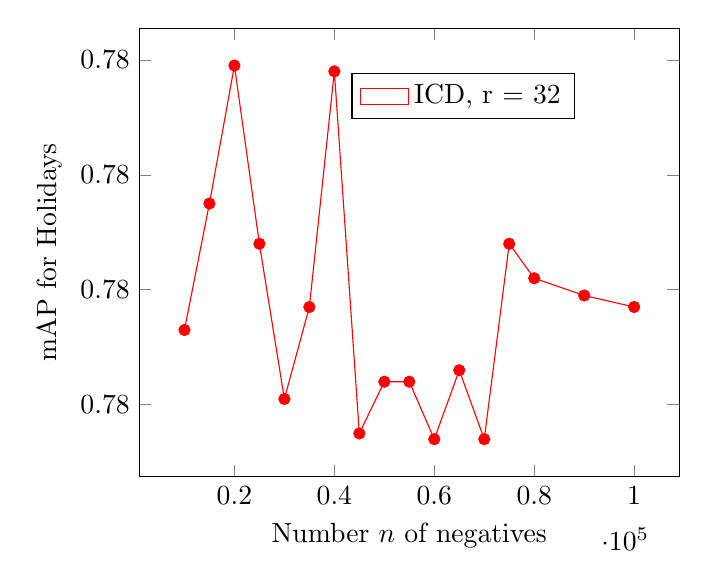
\begin{tikzpicture}
	\begin{axis}[
		xlabel=Number $n$ of negatives,
		ylabel=mAP for Holidays,
		legend style={
			area legend,
			at={(0.6,0.9)},
			anchor=north,
			legend columns=-1}]
%%Poly SLEM
    \addplot[mark=*, red] coordinates{
        (  10000, 0.7773)
        (  15000, 0.7795)
        (  20000, 0.7819)
        (  25000, 0.7788)
        (  30000, 0.7761)
        (  35000, 0.7777)
        (  40000, 0.7818)
        (  45000, 0.7755)
        (  50000, 0.7764)
        (  55000, 0.7764)
        (  60000, 0.7754)
        (  65000, 0.7766)
        (  70000, 0.7754)
        (  75000, 0.7788)
        (  80000, 0.7782)
       (   90000, 0.7779)
       (  100000, 0.7777)
    };
    \addlegendentry{ICD, r = 32}
	\end{axis}
\end{tikzpicture}
\caption{mAP for Holidays using SPoC + Poly SLEM, using ICD and fixed 32-rank.}
\label{icd}
\end{figure}

